\documentclass[border=4mm]{standalone}
\usepackage{tikz}
\usepackage{amsmath}
\usepackage{mathptmx}
\usetikzlibrary{calc}

\begin{document}
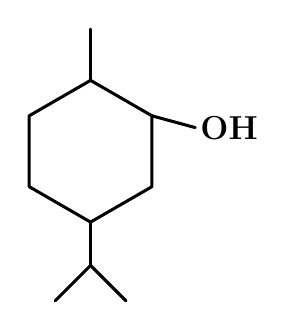
\begin{tikzpicture}[line cap=round, line join=round, line width=1.1pt, font=\fontsize{12}{14}\selectfont]
    \def\r{0.9}
    \coordinate (c1) at (90:\r);
    \coordinate (c2) at (30:\r);
    \coordinate (c3) at (330:\r);
    \coordinate (c4) at (270:\r);
    \coordinate (c5) at (210:\r);
    \coordinate (c6) at (150:\r);
    
    % Vòng 6 cạnh
    \draw (c1) -- (c2) -- (c3) -- (c4) -- (c5) -- (c6) -- cycle;
    
    % Nhánh methyl ở đỉnh trên
    \draw (c1) -- ($(c1)+(0,0.65)$);
    
    % Nhánh OH ở cạnh phải
    \draw (c2) -- ($(c2)+(0.55,-0.15)$) node[right=-2pt] {\textbf{OH}};
    
    % Nhánh isopropyl ở đỉnh dưới
    \draw (c4) -- ($(c4)+(0,-0.55)$) coordinate (iso);
    \draw (iso) -- ($(iso)+(-0.45,-0.45)$);
    \draw (iso) -- ($(iso)+(0.45,-0.45)$);
\end{tikzpicture}
\end{document}
